\documentclass{article}

\usepackage[utf8]{inputenc}
\usepackage{amsmath}
\usepackage{graphicx}
\usepackage{float}
\usepackage{enumerate}
\usepackage[top=1.5cm,left=1.5cm,right=1.5cm,bottom=1.5cm]{geometry}

\begin{document}
\title{\Large La difracción de distintas rendijas como transformada de Fourier de sus respectivas funciones pupila}
\author{Alfredo Ricci\\Juan Andrés Urrea}
\maketitle

\section{La Transformada de Fourier}
Cuando se trabaja con una función, aplicada sobre el dominio temporal, $f(t)$, se le puede aplicar un operador conocido como la \textbf{Transformada de Fourier}, que vendrá definido de distintas maneras dependiendo de la naturaleza de $f(t)$. Existen entonces cuatro casos de $f(t)$ donde se definen las correspondientes transformadas de Fourier de dicha función $f(t)$, ahora llamada $F(\omega)$, cuyo nuevo dominio será la frecuencia. A pesar de sus distintas definiciones, este operador sirve el propósito de enunciar el espectro de frecuencias que compone a $f(t)$. Es decir, genera como resultado una combinación lineal de las diferentes frecuencias incluidas en $f(t)$ para así determinar cuales componen a $f(t)$ y la proporción en la que lo hacen. A continuación se enuncia la definición de dicho operador para dos casos de $f(t)$[2]:
\begin{enumerate}[(a)]
\item $f(t)$: Función discreta de longitud finita N.
\begin{eqnarray*}
X_k=\sum_{n=0}^{N-1} x_n e^{\dfrac{-2\pi ikn}{N}}\\
k=0,1,...,N-1
\end{eqnarray*}
Donde $x_n$ denota el elemento enésimo de la función o arreglo original de longitud N, $X_k$ denota el k-ésimo elemento del arreglo resultante después de realizar la transformada, siendo también de longitud N. 

\item $f(t)$: Fnunción continua de longitud finita.
\begin{eqnarray*}
F(\omega)=\int_{a}^{b} f(t)e^{-2\pi i \omega t}dt
\end{eqnarray*}
Dada que la función $f(t)$ solo existe en un intervalo dado, los límites vendrán dados por los límites inferior y superior de dicho intervalo. 
\end{enumerate}
Estas transfromaciones generan funciones o arreglos en el dominio de la frecuencia que permiten determinar las frecuencias que componen $f(t)$. 

\section{La Transformada de Fourier como Diracción de Una Rejilla Determinada}
La propuesta de experimento planteada tiene como propósito mostrar la correspondencia entre la tranformada de Fourier de una señal \textit{pupila} y el patrón de difracción que se presenta en el campo lejano debido a dicha señal. La mayor parte de la explicación física y matemática se encuentra en [1], sin embargo a continuación se presenta la deducción que permite ver la validez de la correspondencia dicha anteriormente, procedimiento extraído de [1]. Para comenzar, se parte de la integral de difracción de Fresnel-Kirchoff [1]:
\begin{eqnarray*}
U(P)=-\frac{Ai}{\lambda}\frac{\cos \delta}{r\prime s\prime}\int \int_C\frac{e^{ik(r+s)}}{rs}[cos(n,r)-cos(n,s)]dS 
\end{eqnarray*}
Esta integral define la perturbación total en el punto P según la siguiente geometría:

\begin{figure}[H]
\centering
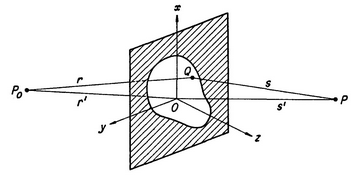
\includegraphics[width=0.8\textwidth]{Diagrama.png}
\caption{Geometría de los puntos analizados y la apertura.[1]} \label{fig:geometria}
\end{figure}

Donde:
\begin{itemize}
\item $\delta$ es el ángulo entre la recta normal a la pantalla y la recta $PP_0$.
\item $n$ es el vector unitario hacia adentro de la curva cerrada que define la apertura.
\item $A$ es una constante.
\end{itemize}
Ahora, dado que se analizará la difracción en campos lejanos, se puede asumir $s=s\prime$ y $r=r\prime$ como separación de los puntos a la rendija, de igual forma que se puede asumir que el término $[cos(n,r)-cos(n,s)]$ de la integral no varía mucho. Por esto, este término de aproxima a $2Cos(\delta)$. Gracias a esto, se puede simplificar la integral anterior a:
\begin{eqnarray}
U(P)=-\frac{Ai}{\lambda}\frac{cos(\delta)}{r\prime s\prime} \int \int_{C} e^{ik(r+s)}dS
\end{eqnarray}
Ahora, dado que se estudia cada punto Q dentro de la rendija, es posible expresar su posición bajo las ccordenadas $\zeta$ y $\eta$ como equivalentes cartesianas de x y y, permaneciendo siempre sobre el plano XY. [1] ofrece las siguientes igualdades:
\begin{eqnarray}
r^2 = (x_0 - \zeta)^2 + (y_0 - \eta)^2 + z_0^2\\
s^2 = (x-\zeta)^2 + (y - \eta)^2 + z_0^2\\
r\prime ^2 = x_0^2 + y_0^2 + z_0^2\\
s\prime ^2 = x^2 + y^2 + z^2
\end{eqnarray}
Siendo $(x,y,z)$ las coordenadas cartesianas que describen la al punto P y $(x_0,y_0,z_0)$ las coordenadas que describen al punto $P_0$. Se presenta también la manera más conveniente de relacionar las variables $r$ y $s$ primadas y no primadas, mostrada a continuación, para luego aprovechar el hecho de que se están analizando campos lejanos, donde $r\prime$ y $s\prime$ tienden a $\infty$.
\begin{eqnarray}
r^2 = r\prime ^2 - 2(x_0\zeta + y_0\eta) + \zeta^2 + \eta^2\\
s^2 = s\prime ^2 - 2(x\zeta + y\eta) + \zeta^2 + \eta^2
\end{eqnarray}
Estas expresiones sirven ahora para realizar una expansión lineal de $r$ y $s$, de la forma siguiente:
\begin{eqnarray}
r \rightarrow r\prime - \dfrac{x_0\zeta_0 + y_0\eta}{r\prime} + \dfrac{\zeta^2 + \eta^2}{2r\prime}+...\\
s \rightarrow s\prime - \dfrac{x\zeta + y\eta}{s\prime} +\dfrac{\zeta^2 + \eta^2}{2s\prime} + ...
\end{eqnarray}
Interpretando las expresiones (8)  y (9) como:
\begin{eqnarray}
r \rightarrow r\prime + f(\zeta,\eta)\\
s \rightarrow s\prime + f(\zeta,\eta) 
\end{eqnarray}
Las expresiones (10) y (11) se pueden reemplazar en la expresión (1) para obtener:
\begin{eqnarray}
U(P)=-\dfrac{iAcos(\delta)}{\lambda}\dfrac{e^{ik(r\prime + s\prime)}}{r\prime s\prime}\int \int_C e^{ikf(\zeta,\eta)}d\zeta d\eta
\end{eqnarray}
Para continuar, [1] analiza la propia función $f(\zeta,\eta)$, expresada como:
\begin{eqnarray}
f(\zeta,\eta)= \dfrac{x_0\zeta_0 + y_0\eta}{r\prime} + \dfrac{\zeta^2 + \eta^2}{2r\prime}+...
\end{eqnarray}
La cual se puede simplificar al nombrar la siguientes coordenadas direccionales:
\begin{eqnarray}
l_0 = -\dfrac{x_0}{r\prime}\\
l=\dfrac{x}{s\prime}\\
m_0=-\dfrac{y_0}{r\prime}\\
m = \dfrac{y}{s\prime}
\end{eqnarray}
(14),(15),(16) y (17) se reemplazan en (13) para obtener:
\begin{eqnarray}
f(\zeta,\eta)=(l_0 - l)\zeta + (m_0-m)\eta + \dfrac{1}{2}\left\lbrace \left( \dfrac{1}{r\prime} + \dfrac{1}{s\prime}\right)(\zeta^2 + \eta^2)\right\rbrace + ...\ 
\end{eqnarray}
Para el caso específico de la difracción de \textbf{Fraunhofer}, los términos que involucran los términos cuadráticos se ignoran, lo que da lugar a reescribir (18) como:
\begin{eqnarray}
f(\zeta,\eta) = (l_0 - l)\zeta + (m_0-m)\eta
\end{eqnarray}
Reemplazando (19) en (12) y estableciendo $p=l-l_0$ y  $q=m-,_0$, se obtiene:
\begin{eqnarray}
U(P)=D\int \int_C e^{-ik(p\zeta + q\eta)}d\zeta d\eta
\end{eqnarray}
Ahora, $k$ se puede reemplazar por $\dfrac{2\pi}{\lambda}$, a la vez que la constante se transforma en la función \textit{pupila}.
\begin{eqnarray}
U(p,q)=\int \int_C G(\eta,\zeta) e^{-i\frac{2\pi}{\lambda}(p\zeta + q\eta)}d\zeta d\eta
\end{eqnarray}
Se puede observar que $U(p,q)$ es ahora la tranformada de Fourier continua bidimensional de $G(\zeta,\eta)$. Esta función \textit{pupila} será entonces una constante dentro de la rendija \textbf{C} y 0 fuera de ella.

\section{Montaje Experimental}
Para la realización de este experimento, se plantea inicialmente el siguiente montaje experimental para la visualización del patrón de difracción de la luz a través de distintos tipos de rendijas. Consiste entonces de una fuente de luz monocromática la cual pasa a través de una rendija de difracción y se puede observar en la pantalla lejana a la rendij el patrón de difracción de campos lejanos. Cada tipo de rendija utilizada representará entonces una diferente función \textit{pupila}.


\begin{figure}[H]
\centering
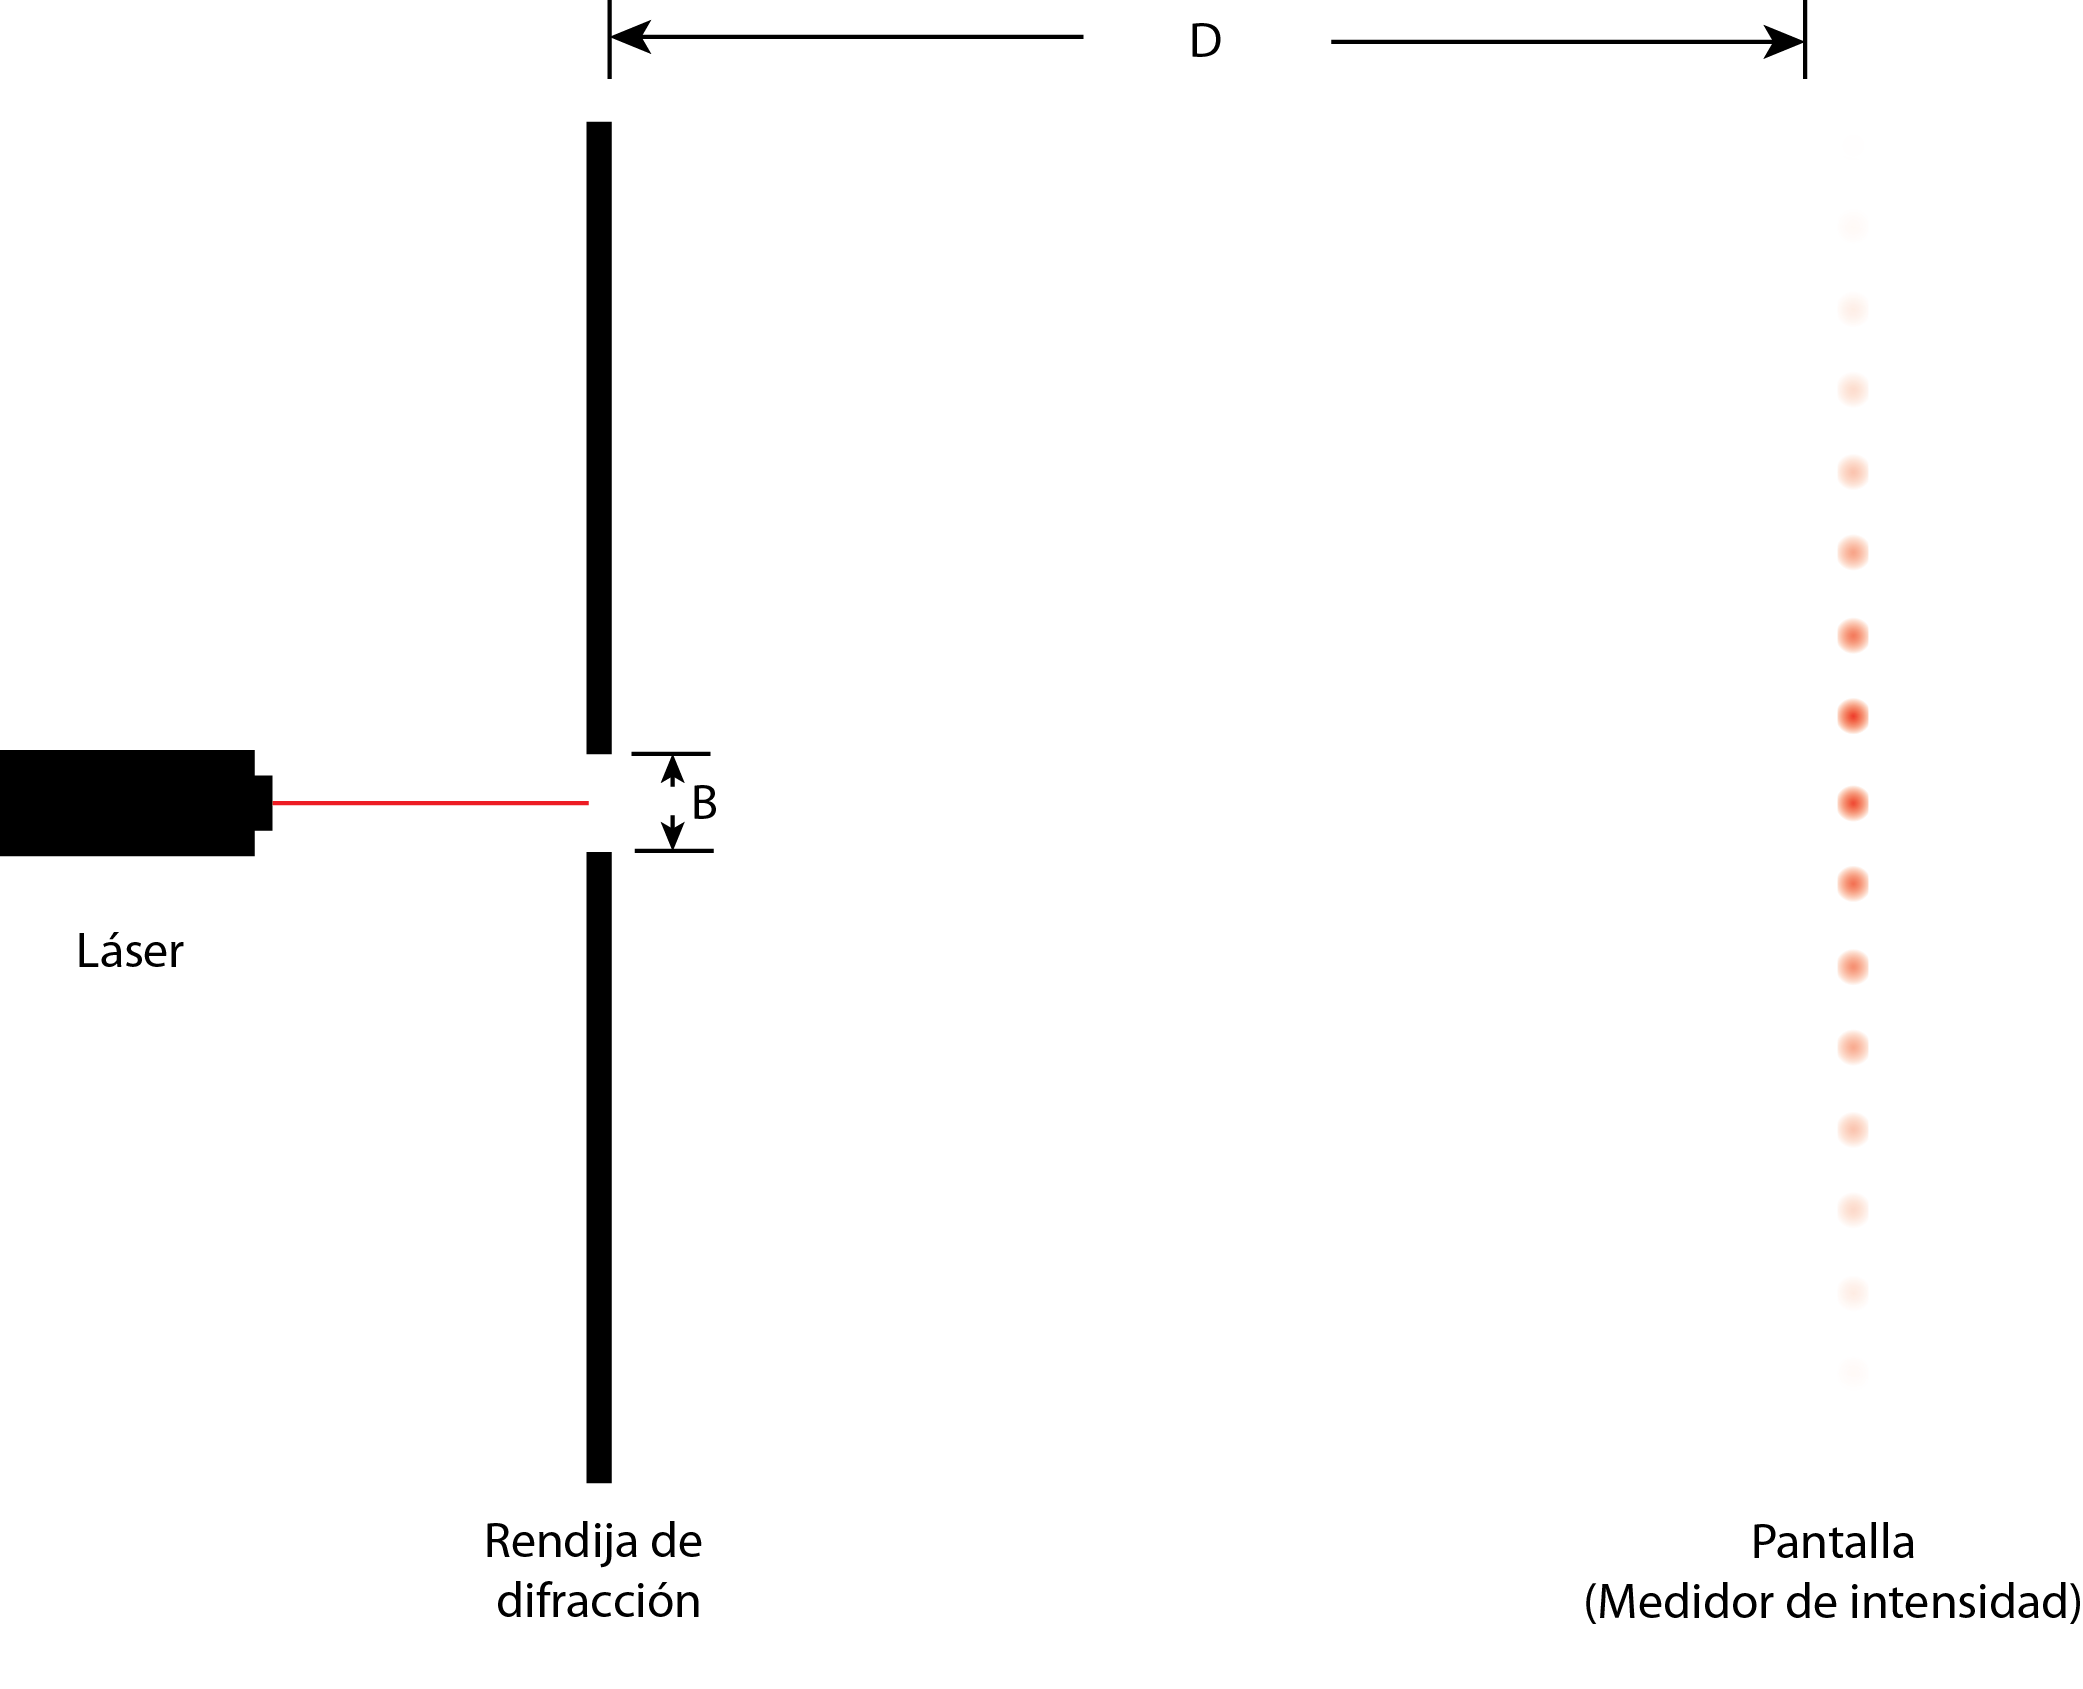
\includegraphics[width=0.55\textwidth]{Montaje.png}
\caption{Montaje propuesto para el experimento} \label{fig:montaje}
\end{figure}

\section{Simulaciones preliminares}
Partiendo de lo establecido en el marco teórico y utilizando el lenguaje de programación científica \textbf{Python} es posible tomar algunos ejemplos de rendijas posibles y modelarlas como funciones \textit{pupila} bidimensionales, matrices cuyos elelmentos son constantes en donde está la apertura y cero donde se bloquea el paso de la luz. Omitiendo el código utilizado por motivos de brevedad más conservándolo para futuras referencias más detalladas, se presentan a continuación algunos de los resultados obtenidos de las simulaciones.

\begin{figure}[H]
\centering
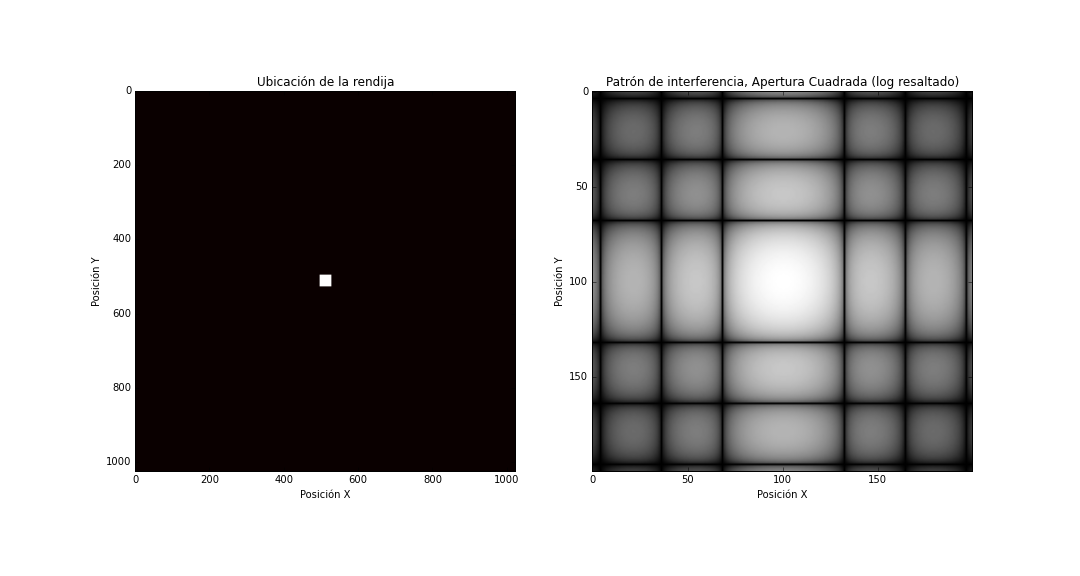
\includegraphics[width=0.98\textwidth]{Cuadrado.png}
\caption{Difracción de una rendija cuadrada} \label{fig:cuadrado}
\end{figure}
\begin{figure}[H]
\centering
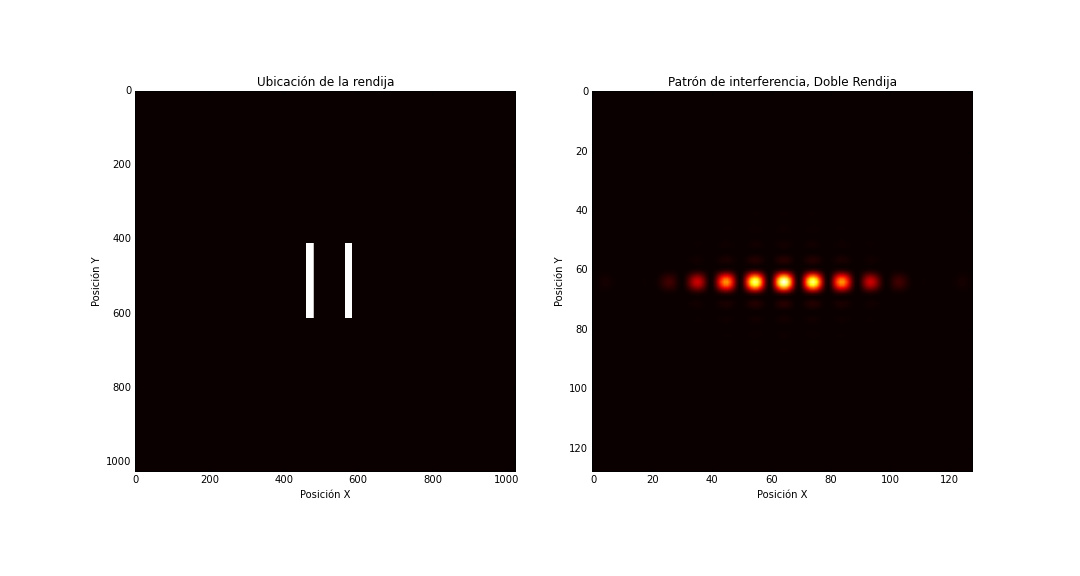
\includegraphics[width=0.98\textwidth]{DosRect.png}
\caption{Difracción de una rendija rectangular doble} \label{fig:rectangulo}
\end{figure}
\begin{figure}[H]
\centering
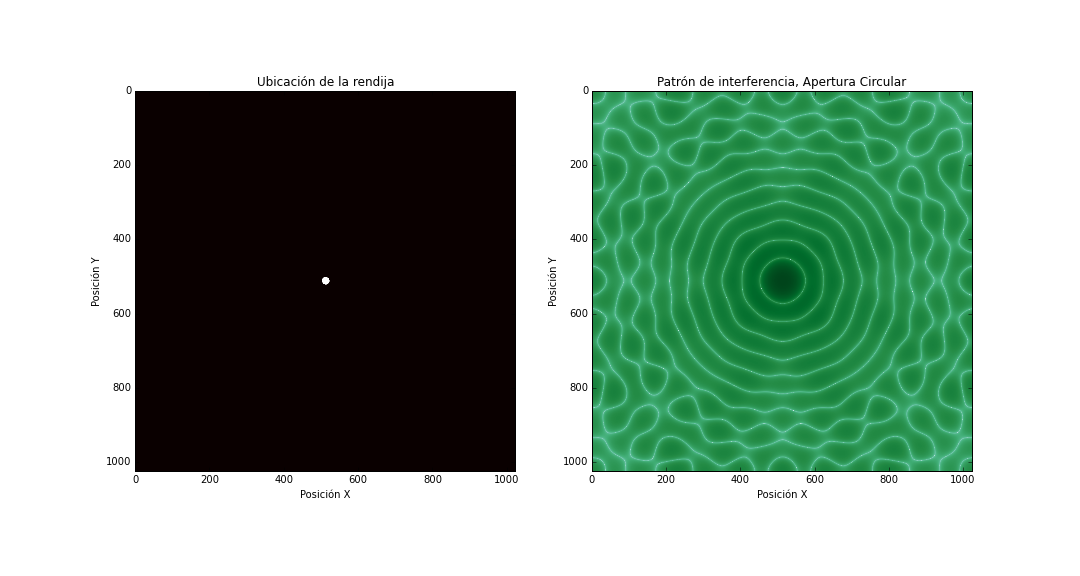
\includegraphics[width=0.98\textwidth]{Circulo.png}
\caption{Difracción de una rendija circular} \label{fig:circulo}
\end{figure}
\section{Bibliografía}
\begin{enumerate}
\item \textbf{Principles of Optics} Born, M. Wolf, E. Fourth Edition. 1970. 
\item  Weisstein, Eric W. "Fourier Transform." From MathWorld--A Wolfram Web Resource.\\ http://mathworld.wolfram.com/FourierTransform.html 
\end{enumerate}
\end{document}